\documentclass[12pt, svgnames, titlepage]{report}

\textwidth=7in
\textheight=9.5in
\topmargin=-1in
\headheight=0in
\headsep=.5in
\hoffset  -.85in


\usepackage{hyperref}
\hypersetup{
    colorlinks,
    citecolor=black,
    filecolor=black,
    linkcolor=black,
    urlcolor=black
}

%\usepackage[T1]{fontenc}
%\usepackage{txfonts}
\usepackage{fancyhdr}
\usepackage{enumitem}
\pagestyle{fancyplain}
\usepackage{xcolor}
\definecolor{UCLABlue}{RGB}{83, 104, 149}
\definecolor{UCLAGold}{RGB}{254, 187, 54}

% Some characters were not being rendered correctly at work
\DeclareUnicodeCharacter{2217}{*}
\DeclareUnicodeCharacter{200B}{ }


\author{Philip Tracton}
\date{\today}
\date{}

\usepackage{tikz}
\usepackage{verbatim}
\usepackage{kpfonts}
\usepackage[explicit]{titlesec}
\newcommand*\chapterlabel{}
\titleformat{\chapter}
  {\gdef\chapterlabel{}
   \normalfont\sffamily\Huge\bfseries\scshape}
  {\gdef\chapterlabel{\thechapter\ }}{0pt}
  {\begin{tikzpicture}[remember picture,overlay]
    \node[yshift=-3cm] at (current page.north west)
      {\begin{tikzpicture}[remember picture, overlay]
        \draw[fill=UCLABlue] (0,0) rectangle
          (\paperwidth,3cm);
        \node[anchor=east,xshift=.9\paperwidth,rectangle,
              rounded corners=20pt,inner sep=11pt,
              fill=UCLAGold]
              {\color{white}\chapterlabel#1};
       \end{tikzpicture}
      };
   \end{tikzpicture}
  }
\titlespacing*{\chapter}{0pt}{50pt}{-60pt}

\usepackage{changepage}
\newenvironment{restoretext}%
    {\@parboxrestore%
     \begin{adjustwidth}{}{\leftmargin}%
    }{\end{adjustwidth}
     }

\lfoot{\colorbox{UCLABlue}{\textcolor{white}{P. Tracton}}}
\cfoot{\colorbox{UCLABlue}{\textcolor{white}{Machine Learning}}}
\rfoot{\colorbox{UCLABlue}{\textcolor{white}{\thepage}}}


\usepackage{array}
\newcolumntype{L}[1]{>{\raggedright\let\newline\\\arraybackslash\hspace{0pt}}m{#1}}

\usepackage{graphicx}
% https://www.overleaf.com/learn/latex/Inserting_Images
\graphicspath{ {./plantuml/uml/} }
\usepackage[export]{adjustbox}

% For math and matrix work
\usepackage{amsmath}

% Use multicol for when we want to show matlab and python code
% side by side doing the same things
\usepackage{multicol}
%\setlength{\columnsep}{1cm}

% use minted for formatting and highlighting code examples
\usepackage{minted}
%\setminted{fontsize=\Large,baselinestretch=1}
% Use a pale grey background for the code
\definecolor{Background}{RGB}{240, 240, 240}

% https://tex.stackexchange.com/questions/27802/set-noindent-for-entire-file/27804
\setlength\parindent{0pt}

% American Math Society Symbols package
\usepackage{amssymb}

\newmintedfile[matlabcode]{matlab}{
bgcolor=Background,
fontfamily=tt,
linenos=true,
numberblanklines=true,
numbersep=5pt,
gobble=0,
frame=leftline,
framerule=0.4pt,
framesep=2mm,
funcnamehighlighting=true,
tabsize=4,
obeytabs=false,
mathescape=false
samepage=false, %with this setting you can force the list to appear on the same page
showspaces=false,
showtabs =false,
texcl=false,
breaklines=true,
}

\newmintedfile[pythoncode]{python}{
bgcolor=Background,
fontfamily=tt,
linenos=true,
numberblanklines=true,
numbersep=5pt,
gobble=0,
frame=leftline,
framerule=0.4pt,
framesep=2mm,
funcnamehighlighting=true,
tabsize=4,
obeytabs=false,
mathescape=false
samepage=false, %with this setting you can force the list to appear on the same page
showspaces=false,
showtabs =false,
texcl=false,
breaklines=true,
}


\title{My Notes for Machine Learning}

\begin{document}
\maketitle
\newpage

\vspace{10mm}
\tableofcontents
\newpage

\chapter{Math Review}
\vspace{10mm}

\section{Linear Algebra}

\subsection{Matrix}

A matrix is a 2-dimensional array of numbers.\\

\textbf{N} is number of rows.  \textbf{M} is number of columns.\\

Matrices are specified as NxM.\\

$A_{ij}$ is how you specify a single location in a matrix.  It is row I and column J.



\begin{equation}
  \textbf{A} = \left[
    \begin{matrix}
      x_{11} & x_{12} & x_{13} & \dots  & x_{1m} \\
      x_{21} & x_{22} & x_{23} & \dots  & x_{2m} \\
      \vdots & \vdots & \vdots & \ddots & \vdots \\
      x_{N1} & x_{N2} & x_{N3} & \dots  & x_{NM}
    \end{matrix}
    \right]
  \label{eqn:BasicMatrix}
\end{equation}

A vector is a matrix with one column and many rows and specified as Nx1\\

$v_i$ is the $i^{th}$ element of the vector V.\\

\begin{equation}
  \textbf{{v}} = \left[
    \begin{matrix}
      x_{0} \\
      x_{1} \\
      x_{2} \\
      \vdots \\
      x_{N}
    \end{matrix}
    \right]
  \label{eqn:BasicVector}
\end{equation}

Matrices are usually denoted by uppercase names while vectors are lowercase.\\

\textbf{Scalar} means that an object is a single value, not a vector or matrix.\\

$\mathbb{R}$ refers to the set of scalar real numbers.\\

$\mathbb{R}^{n}$ refers to the set of n-dimensional vectors of real numbers.\\


\newpage
\underline{\href{http://www.mathworks.com}{Matlab}} (or \underline{\href{https://www.gnu.org/software/octave/}{Octave}}) and \underline{\href{http://www.python.org}{Python}} are 2 very common languages for doing machine learning and math work in general.  They are very different languages.  Matlab is a number crunching specific language.  This is pretty much all it does.  Python is a general purpose language with a lot of built up libraries, \underline{\href{https://numpy.org/}{Numpy}} in particular,  to support doing this type of work.\\

This document will try to go over all concepts in both languages in order to better understand how the math works from 2 different perspectives.\\

One of the issues to keep track of is that Matlab starts counting at 1 and Python starts counting at 0!  Notice in the code below that A(2,3) in Matlab will get you the same location as A[1][2] in Python for the same matrices\\

\begin{multicols}{2}
  [
    This is an example of creating a simple 3x3 matrix in both Matlab and Python.  Notice that Matlab is a little bit simpler.  There is no need to import a library for it.  Python doesn't need one either technically, but numpy will be used a lot for machine learning work and we should just start with it.\\
  ]
  Matlab\\
  \matlabcode{matlab/matrix.m}
  \columnbreak

  Python\\
  \pythoncode{python/matrix.py}
  
\end{multicols}

\subsection{Matrix Operations}
\subsubsection{Addition and Subtraction}
Addition and subtraction are element-wise, so you simply add or subtract each corresponding element:\\
To add or subtract two matrices, their dimensions must be the \textbf{same}.\\

\begin{equation}
  \left[
    \begin{matrix}
      a & b \\
      c & d
    \end{matrix}
    \right] +
  \left[
    \begin{matrix}
      w & x \\
      y & z
    \end{matrix}
    \right]=
  \left[
    \begin{matrix}
      a+w & b+x \\
      c+y & d+z
    \end{matrix}
    \right]
  \label{eqn:MatrixAddition}
\end{equation}

\begin{multicols}{2}
  Matlab\\
  \matlabcode{matlab/matrix_addition.m}
  \columnbreak

  Python\\
  \pythoncode{python/matrix_addition.py}
  
\end{multicols}

\begin{equation}
  \left[
    \begin{matrix}
      a & b \\
      c & d
    \end{matrix}
    \right] -
  \left[
    \begin{matrix}
      w & x \\
      y & z
    \end{matrix}
    \right]=
  \left[
    \begin{matrix}
      a-w & b-x \\
      c-y & d-z
    \end{matrix}
    \right]
  \label{eqn:MatrixSubtraction}
\end{equation}

\begin{multicols}{2}
  Matlab\\
  \matlabcode{matlab/matrix_subtraction.m}
  \columnbreak

  Python\\
  \pythoncode{python/matrix_subtraction.py}
  
\end{multicols}

For matrix addition/subtraction there is not much of a difference.  Python takes a little more set up in that you need to import numpy, but the actual operational step is identical.

\subsubsection{Scalar Multiplication and Division}
In scalar multiplication, we simply multiply every element by the scalar value:
\begin{equation}
  \left[
    \begin{matrix}
      a & b \\
      c & d
    \end{matrix}
    \right] * x =
  \left[
    \begin{matrix}
      a*x & b*x \\
      c*x & d*x
    \end{matrix}
    \right]
  \label{eqn:MatrixScalarMultiplication}
\end{equation}

In scalar division, we simply divide every element by the scalar value:
\begin{equation}
  \left[
    \begin{matrix}
      a & b \\
      c & d
    \end{matrix}
    \right] / x =
  \left[
    \begin{matrix}
      a/x & b/x \\
      c/x & d/x
    \end{matrix}
    \right]
  \label{eqn:MatrixScalarMultiplication}
\end{equation}

\begin{multicols}{2}
  Matlab\\
  \matlabcode{matlab/matrix_scalar_mult_div.m}
  \columnbreak

  Python\\
  \pythoncode{python/matrix_scalar_mult_div.py}
  
\end{multicols}

\subsubsection{Matrix Vector Multiplication}
The result is a \textbf{vector}. The number of \textbf{columns} of the matrix must equal the number of \textbf{rows} of the vector.\\

An \textbf{m x n matrix} multiplied by an \textbf{n x 1} vector results in an \textbf{m x 1} vector.\\

Some more \underline{\href{https://mathinsight.org/matrix_vector_multiplication}{Math Insights}} \\

Below is an example of a matrix-vector multiplication. Make sure you understand how the multiplication works. \\

\begin{equation}
  \left[
    \begin{matrix}
      a & b \\
      c & d \\
      e & f 
    \end{matrix}
    \right] *
  \left[
    \begin{matrix}
      x\\
      y\\
    \end{matrix}
    \right]=
  \left[
    \begin{matrix}
      a*x + b*y \\
      c*x + d*y\\
      e*x + f*y
    \end{matrix}
    \right]
  \label{eqn:MatrixVectorMultiplication}
\end{equation}


\subsubsection{Matrix Matrix Multiplication}

This is also known as the \underline{\href{https://www.mathsisfun.com/algebra/vectors-dot-product.html}{dot product}}.\\

An \textbf{m x n} matrix multiplied by an \textbf{n x o} matrix results in an \textbf{m x o} matrix. In the example, a 3 x 2 matrix times a 2 x 2 matrix resulted in a 3 x 2 matrix.\\

To multiply two matrices, the number of columns of the first matrix must equal the number of rows of the second matrix.  The process is to take each row of the first matrix and multiply it by each column of the second matrix.  Iterate this through each row in the first matrix with each column in the second matrix.  \\

You can \textbf{NOT} reverse the order.  $\textbf{A}*\textbf{B}$ is not $\textbf{B}*\textbf{A}$\\
Multiplication is associative.  $(\textbf{A}*\textbf{B})*\textbf{C} = \textbf{A}*(\textbf{B}*\textbf{C})$\\

\begin{equation}
  \left[
    \begin{matrix}
      a & b \\
      c & d \\
      e & f
    \end{matrix}
    \right] *
  \left[
    \begin{matrix}
      w & x \\
      y & z
    \end{matrix}
    \right]=
  \left[
    \begin{matrix}
      a*w + b*y  & a*x + b*z\\
      c*w + d*y  & c*x + d*z\\
      e*w + f*y  & e*x + f*z
    \end{matrix}
    \right]
  \label{eqn:MatrixMatrixMultiplication}
\end{equation}

\begin{multicols}{2}
  Matlab\\
  \matlabcode{matlab/matrix_matrix_multiplication.m}
  \columnbreak

  Python\\
  \pythoncode{python/matrix_matrix_multiplication.py}
  
\end{multicols}

Notice the syntax is starting to differ more.  For Matlab, you can just multiply the vectors like any other variable.  In python we need to use the \underline{\href{https://docs.scipy.org/doc/numpy/reference/generated/numpy.dot.html}{dot method}}.  Notice it is A that calls dot with B as a parameter.

\subsubsection{Identity}

The identity matrix is a square matrix (m=n) that has 1's along the diagnal and zeros everywhere else and is usually denoted by the letter \textbf{I}.

The identity matrix, when multiplied by any matrix of the same dimensions, results in the original matrix. It's just like multiplying numbers by 1. The identity matrix simply has 1's on the diagonal (upper left to lower right diagonal) and 0's elsewhere.\\

When multiplying the identity matrix after some matrix ($A∗I$), the square identity matrix's dimension should match the other matrix's \textbf{columns}. When multiplying the identity matrix before some other matrix (I∗A), the square identity matrix's dimension should match the other matrix's \textbf{rows}.\\

\begin{equation}
  \textbf{I} = \left[
    \begin{matrix}
      1 & 0 & 0 & \dots  & 0 \\
      0 & 1 & 0 & \dots  & 0 \\
      \vdots & \vdots & \vdots & \ddots & \vdots \\
      0 & 0 & 0 & \dots  & 1
    \end{matrix}
    \right]
  \label{eqn:IdentityMatrix}
\end{equation}

\newpage
\begin{multicols}{2}
  Matlab\\
  \matlabcode{matlab/matrix_identity.m}
  \columnbreak

  Python\\
  \pythoncode{python/matrix_identity.py}
  
\end{multicols}

Again the syntax is still mostly the same.  Matlab multiplies are calls to the dot method in Python.  The \underline{\href{https://www.mathworks.com/help/matlab/ref/eye.html}{eye()}} function in Matlab does the same thing as the numpy version of \underline{\href{https://docs.scipy.org/doc/numpy/reference/generated/numpy.eye.htm}{eye()}}.  The difference is that in Matlab it is a built in function and in Python you need to call the method inside the Numpy library.

\subsubsection{Transpose}

The \textbf{transposition} of a matrix is like rotating the matrix 90° in clockwise direction and then reversing it. We can compute transposition of matrices in matlab with the transpose(A) function or A'\\

In other words: $A_{ij} = A^T_{ji}$  \\

​\begin{multicols}{2}
  Matlab\\
  \matlabcode{matlab/matrix_transpose.m}
  \columnbreak
  
  Python\\
  \pythoncode{python/matrix_transpose.py}
  
\end{multicols}	

In Matlab the ' operator will transpose a matrix.  There is a \underline{\href{https://www.mathworks.com/help/matlab/ref/transpose.html}{transpose}} function in Matlab but the ' notation is very common and easier.\\

In Python we must call the \underline{\href{https://docs.scipy.org/doc/numpy/reference/generated/numpy.ndarray.transpose.html}{transpose method}} on our matrix.\\

\subsubsection{Inverse}

The inverse of a matrix A is denoted $A^{-1}$.
Multiplying by the inverse results in the identity matrix.  \\

\begin{equation}
I = A*A^{-1}
\end{equation}

A non square matrix does not have an inverse matrix. We can compute inverses of matrices in Octave with the \underline{\href{https://octave.sourceforge.io/octave/function/pinv.html}{pinv(A)}} function and in Matlab with the \underline{\href{https://www.mathworks.com/help/matlab/ref/inv.html}{inv(A)}} function. Matrices that don't have an inverse are \underline{\href{http://mathworld.wolfram.com/SingularMatrix.html}{singular}} or \underline{\href{https://www.encyclopediaofmath.org/index.php/Degenerate_matrix}{degenerate}}. \\

\newpage
​ \begin{multicols}{2}
  Matlab\\
  \matlabcode{matlab/matrix_inverse.m}
  \columnbreak

  Python\\
  \pythoncode{python/matrix_inverse.py}

\end{multicols}	

  The Matlab code is pretty straight forward.  You can call the inv() function on a matrix.  You can multiply the original matrix by its inverse and get the identity.\\

  In Python it is a little more complicated.  We need to bring in the numpy \underline{\href{https://docs.scipy.org/doc/numpy/reference/routines.linalg.html}{Linear Algebra}} library.  Once this library is brought in, we can use the \underline{\href{https://docs.scipy.org/doc/numpy/reference/generated/numpy.linalg.inv.html\#numpy.linalg.inv}{inv()}} method in it on our matrix.  From there we can do all the same things as in Matlab but with our Python syntax.\\
  

\section{Calculus}

\section{Probability}
\section{Statistics}


\chapter{Introduction to Machine Learning}
\vspace{10mm}
\section{Introduction to Machine Learning}


Machine Learning: Field of study that gives computers the ability to learn without being explicitly programmed. \\

Well-posed Learning Problem: A computer program is said to learn from experience E with respect to some task T and some performance measure P, if its performance on T, as measured by P, improves with experience E. \\

Machine Learning Algorithms
\begin{itemize}
\item Supervised Learning
\item Unsupervised Learning
\item Reinforcement Learning
\item Recommender Systems
\end{itemize}


\subsection{Supervised Learning}

In supervised learning, we are given a data set and already know what our correct output should look like, having the idea that there is a relationship between the input and the output.\\

Supervised learning problems are categorized into "regression" and "classification" problems. In a regression problem, we are trying to predict results within a continuous output, meaning that we are trying to map input variables to some continuous function. In a classification problem, we are instead trying to predict results in a discrete output. In other words, we are trying to map input variables into discrete categories. \\

In \textbf{supervised learning}, the "right answers" are known.\\

A \textbf{Regression} is predicting a value! For example Given a picture of a person, we have to predict their age on the basis of the given picture\\

A \textbf{classification} is breaking into groups or discrete values.  For example Given a patient with a tumor, we have to predict whether the tumor is malignant or benign.\\


\subsection{Unsupervised Learning}

In \textbf{unsupervised learning}, the "right answers" are \textbf{not} known.\\



Unsupervised learning allows us to approach problems with little or no idea what our results should look like. We can derive structure from data where we don't necessarily know the effect of the variables.\\

We can derive this structure by clustering the data based on relationships among the variables in the data.\\

With unsupervised learning there is no feedback based on the prediction results. \\

\subsection{Model}

Input variables or input features are denoted as $x^{(i)}$\\
Output or target variable we are trying to predict are denoted as $y^{(i)}$\\
The pair $(x^{(i)}, y^{(i)})$ is called a training example.\\

To establish notation for future use, we’ll use $x^{(i)}$ to denote the \textbf{“input”} variables (living area in this example), also called input features, and $y^{(i)}$ to denote the \textbf{“output”} or target variable that we are trying to predict (price). A pair $(x^{(i)}, y^{(i)})$ is called a \textbf{training example}, and the dataset that we’ll be using to learn—a list of m training examples $(x^{(i)}, y^{(i)})$; i=1,...,m—is called a \textbf{training set}. Note that the superscript “(i)” in the notation is simply an index into the training set, and has nothing to do with exponentiation. We will also use \textbf{X} to denote the space of input values, and \textbf{Y} to denote the space of output values. In this example, X = Y = $\mathbb{R}$.

To describe the supervised learning problem slightly more formally, our goal is, given a training set, to learn a function
\begin{equation}
  h : X \rightarrow Y
\end{equation}
so that h(x) is a “good” predictor for the corresponding value of y. For historical reasons, this function h is called a hypothesis. Seen pictorially, the process is therefore like this:

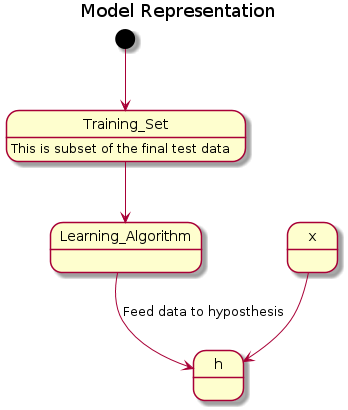
\includegraphics{model_representation.png}

When the target variable that we’re trying to predict is continuous, such as in our housing example, we call the learning problem a regression problem. When y can take on only a small number of discrete values (such as if, given the living area, we wanted to predict if a dwelling is a house or an apartment, say), we call it a classification problem. \\

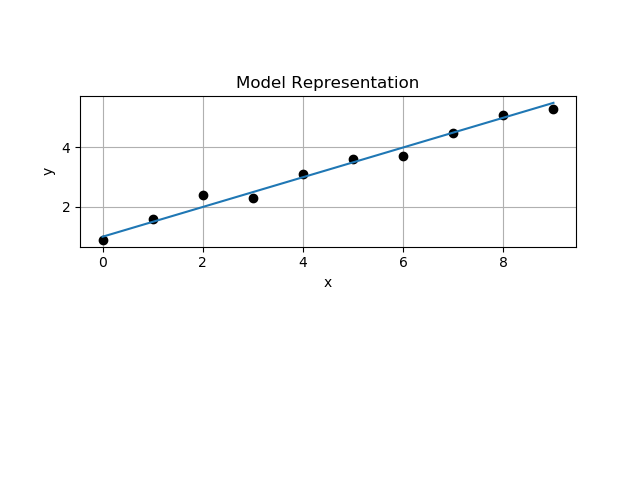
\includegraphics{python/model_plot_representation.png}\\

This is an attempt at a linear fit for this data.  It is not quite a match, but it is very close.  The plot for the line is $y=0.5x+1$ which is our hypothesis fuction h. 


\subsection{Cost Functions}

We can measure the accuracy of our hypothesis function by using a \textbf{cost function}. This takes an average difference (actually a fancier version of an average) of all the results of the hypothesis with inputs from x's and the actual output y's. \\

\begin{equation}
J(\theta_{0}, \theta_{1}) = \frac{1}{2m} \sum_{i=1}^{m} (\hat{y} -y^{i})^{2} = \frac{1}{2m} \sum_{i=1}^{m} (h_{\theta}(x^{i})-y^{i})^2
\end{equation}

m is the number of training examples. The goal is to minimize $J(\theta_{0}, \theta_{1})$.

To break it apart, it is $\frac{1}{2} \bar{x}$ where $\bar{x}$ is the mean of the squares of $h_{\theta}(x^{i}) -y^{i}$, or the difference between the predicted value and the actual value.\\

This function is otherwise called the \textbf{Squared error function}, or \textbf{Mean squared error}. The mean is halved $\frac{1}{2}$ as a convenience for the computation of the gradient descent, as the derivative term of the square function will cancel out the $\frac{1}{2}$ term. \\

For our previous example of $y=0.5x + 1$, we have $h_{\theta}(x^{i}) = \theta_{0} + \theta_{1}x^{i}$.  This leads to our cost function of 

\begin{equation}
J(\theta_{0}, \theta_{1}) = \frac{1}{2m} \sum_{i=1}^{m} (\theta_{0} + \theta_{1}x^{i} - y^{i})^{2} 
\end{equation}

Choose $\theta_{0}, \theta_{1}$ so that $h_{\theta}(x)$ is close to $y$ for training examples $(x,y)$\\

\textbf{KEY NOTE:} The cost function calculates a single value based on a specific $\theta_{0}, \theta_{1}$ pair.  It does not find the best $\theta_{0}, \theta_{1}$ values.  These values are supplied.  Gradient Descent is the process of finding the best $\theta_{0}, \theta_{1}$ values.

\newpage
\begin{multicols}{2}
  [
    This is a cost function implementation for the simple linear equation of $h_{theta}(x) = \theta_{0} + \theta_{1}x$
  ]
  Matlab\\
  \matlabcode{matlab/cost_function.m}
  \columnbreak

  Python\\
  \pythoncode{python/cost_function.py}
  
\end{multicols}

\newpage
\begin{multicols}{2}
  [
    These are the test scripts for driving the cost\_function implementations.  Both are fed the same input data and come back with the same cost value of 0.019.
  ]
  Matlab\\
  \matlabcode{matlab/test_cost_function.m}
  \columnbreak

  Python\\
  \pythoncode{python/test_cost_function.py}
  
\end{multicols}

\newpage
\begin{multicols}{2}
  [
    This is an example of trying different values for $\theta_{0} and \theta_{1}$ and plotting the results.
  ]
  Matlab\\
  \matlabcode{matlab/plot_cost_function.m}
  \columnbreak

  Python\\
  \pythoncode{python/plot_cost_function.py}
  
\end{multicols}

This is the graph created by python, which looks better than the one from Matlab/Octave.  There are 3 line and circles for the actual data.  The first line is the blue one across the X-Axis since we are using 0,0.  The best fit line in red has the ideal value for minimizing cost.  The last line shows it being close, but a little off.\\

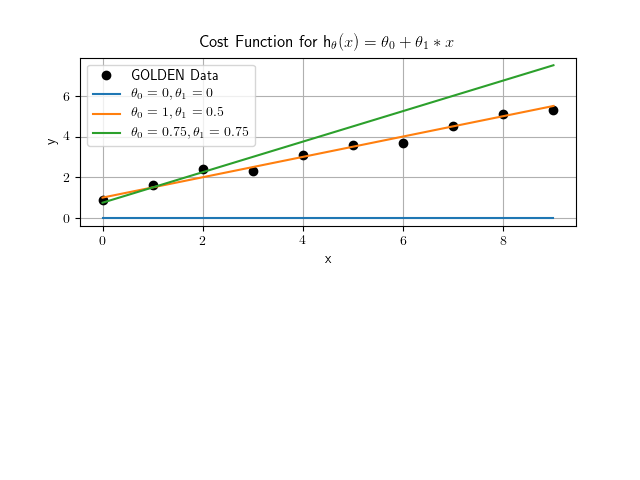
\includegraphics{python/plot_cost_function.png}\\



\end{document}
